% Options for packages loaded elsewhere
% Options for packages loaded elsewhere
\PassOptionsToPackage{unicode}{hyperref}
\PassOptionsToPackage{hyphens}{url}
\PassOptionsToPackage{dvipsnames,svgnames,x11names}{xcolor}
%
\documentclass[
  12pt,
]{article}
\usepackage{xcolor}
\usepackage[margin=2.5cm,top=3cm,bottom=3cm]{geometry}
\usepackage{amsmath,amssymb}
\setcounter{secnumdepth}{5}
\usepackage{iftex}
\ifPDFTeX
  \usepackage[T1]{fontenc}
  \usepackage[utf8]{inputenc}
  \usepackage{textcomp} % provide euro and other symbols
\else % if luatex or xetex
  \usepackage{unicode-math} % this also loads fontspec
  \defaultfontfeatures{Scale=MatchLowercase}
  \defaultfontfeatures[\rmfamily]{Ligatures=TeX,Scale=1}
\fi
\usepackage{lmodern}
\ifPDFTeX\else
  % xetex/luatex font selection
  \setmainfont[]{Times New Roman}
\fi
% Use upquote if available, for straight quotes in verbatim environments
\IfFileExists{upquote.sty}{\usepackage{upquote}}{}
\IfFileExists{microtype.sty}{% use microtype if available
  \usepackage[]{microtype}
  \UseMicrotypeSet[protrusion]{basicmath} % disable protrusion for tt fonts
}{}
\usepackage{setspace}
\makeatletter
\@ifundefined{KOMAClassName}{% if non-KOMA class
  \IfFileExists{parskip.sty}{%
    \usepackage{parskip}
  }{% else
    \setlength{\parindent}{0pt}
    \setlength{\parskip}{6pt plus 2pt minus 1pt}}
}{% if KOMA class
  \KOMAoptions{parskip=half}}
\makeatother
% Make \paragraph and \subparagraph free-standing
\makeatletter
\ifx\paragraph\undefined\else
  \let\oldparagraph\paragraph
  \renewcommand{\paragraph}{
    \@ifstar
      \xxxParagraphStar
      \xxxParagraphNoStar
  }
  \newcommand{\xxxParagraphStar}[1]{\oldparagraph*{#1}\mbox{}}
  \newcommand{\xxxParagraphNoStar}[1]{\oldparagraph{#1}\mbox{}}
\fi
\ifx\subparagraph\undefined\else
  \let\oldsubparagraph\subparagraph
  \renewcommand{\subparagraph}{
    \@ifstar
      \xxxSubParagraphStar
      \xxxSubParagraphNoStar
  }
  \newcommand{\xxxSubParagraphStar}[1]{\oldsubparagraph*{#1}\mbox{}}
  \newcommand{\xxxSubParagraphNoStar}[1]{\oldsubparagraph{#1}\mbox{}}
\fi
\makeatother


\usepackage{longtable,booktabs,array}
\usepackage{calc} % for calculating minipage widths
% Correct order of tables after \paragraph or \subparagraph
\usepackage{etoolbox}
\makeatletter
\patchcmd\longtable{\par}{\if@noskipsec\mbox{}\fi\par}{}{}
\makeatother
% Allow footnotes in longtable head/foot
\IfFileExists{footnotehyper.sty}{\usepackage{footnotehyper}}{\usepackage{footnote}}
\makesavenoteenv{longtable}
\usepackage{graphicx}
\makeatletter
\newsavebox\pandoc@box
\newcommand*\pandocbounded[1]{% scales image to fit in text height/width
  \sbox\pandoc@box{#1}%
  \Gscale@div\@tempa{\textheight}{\dimexpr\ht\pandoc@box+\dp\pandoc@box\relax}%
  \Gscale@div\@tempb{\linewidth}{\wd\pandoc@box}%
  \ifdim\@tempb\p@<\@tempa\p@\let\@tempa\@tempb\fi% select the smaller of both
  \ifdim\@tempa\p@<\p@\scalebox{\@tempa}{\usebox\pandoc@box}%
  \else\usebox{\pandoc@box}%
  \fi%
}
% Set default figure placement to htbp
\def\fps@figure{htbp}
\makeatother





\setlength{\emergencystretch}{3em} % prevent overfull lines

\providecommand{\tightlist}{%
  \setlength{\itemsep}{0pt}\setlength{\parskip}{0pt}}



 


\usepackage{booktabs}
\usepackage{caption}
\usepackage{longtable}
\usepackage{colortbl}
\usepackage{array}
\usepackage{anyfontsize}
\usepackage{multirow}
\usepackage[noblocks]{authblk}
\renewcommand*{\Authsep}{, }
\renewcommand*{\Authand}{, }
\renewcommand*{\Authands}{, }
\renewcommand\Affilfont{\small}
\makeatletter
\@ifpackageloaded{caption}{}{\usepackage{caption}}
\AtBeginDocument{%
\ifdefined\contentsname
  \renewcommand*\contentsname{Table of contents}
\else
  \newcommand\contentsname{Table of contents}
\fi
\ifdefined\listfigurename
  \renewcommand*\listfigurename{List of Figures}
\else
  \newcommand\listfigurename{List of Figures}
\fi
\ifdefined\listtablename
  \renewcommand*\listtablename{List of Tables}
\else
  \newcommand\listtablename{List of Tables}
\fi
\ifdefined\figurename
  \renewcommand*\figurename{Figure}
\else
  \newcommand\figurename{Figure}
\fi
\ifdefined\tablename
  \renewcommand*\tablename{Table}
\else
  \newcommand\tablename{Table}
\fi
}
\@ifpackageloaded{float}{}{\usepackage{float}}
\floatstyle{ruled}
\@ifundefined{c@chapter}{\newfloat{codelisting}{h}{lop}}{\newfloat{codelisting}{h}{lop}[chapter]}
\floatname{codelisting}{Listing}
\newcommand*\listoflistings{\listof{codelisting}{List of Listings}}
\makeatother
\makeatletter
\makeatother
\makeatletter
\@ifpackageloaded{caption}{}{\usepackage{caption}}
\@ifpackageloaded{subcaption}{}{\usepackage{subcaption}}
\makeatother
\makeatletter
\@ifpackageloaded{tcolorbox}{}{\usepackage[skins,breakable]{tcolorbox}}
\makeatother
\makeatletter
\@ifundefined{shadecolor}{\definecolor{shadecolor}{HTML}{31BAE9}}{}
\makeatother
\makeatletter
\makeatother
\makeatletter
\ifdefined\Shaded\renewenvironment{Shaded}{\begin{tcolorbox}[boxrule=0pt, borderline west={3pt}{0pt}{shadecolor}, interior hidden, frame hidden, enhanced, breakable, sharp corners]}{\end{tcolorbox}}\fi
\makeatother
\usepackage{bookmark}
\IfFileExists{xurl.sty}{\usepackage{xurl}}{} % add URL line breaks if available
\urlstyle{same}
\hypersetup{
  pdftitle={Actitudes hacia la Violencia Política: Educación, Clase y Participación en Protestas en Chile (2016-2023)},
  pdfauthor={René Canales},
  colorlinks=true,
  linkcolor={blue},
  filecolor={Maroon},
  citecolor={blue},
  urlcolor={blue},
  pdfcreator={LaTeX via pandoc}}


\title{Actitudes hacia la Violencia Política: Educación, Clase y
Participación en Protestas en Chile (2016-2023)}
\author{René Canales}
\date{}
\begin{document}
\maketitle
\begin{abstract}
\textbf{Keywords}: Political Violence, Protest Participation, Education,
Social Class, Chile
\end{abstract}


\setstretch{1.5}
\section{Antecedentes}\label{antecedentes}

El 18 de octubre de 2019 marcó un antes y un después en la historia
política de Chile. Lo que comenzó como una evasión masiva del metro en
Santiago se transformó en pocas horas en el acontecimiento contencioso
más importante desde el retorno a la democracia en 1990 (Somma et al.,
2021). Durante semanas, miles de personas ocuparon las calles de todo el
país, desafiando no solo la herencia del neoliberalismo que arrastraba
el país desde la dictadura, sino también los límites históricos de lo
que se consideraba acción colectiva. Las protestas del llamado
``estallido social'' combinaron masividad, aparente transversalidad
social y repertorios confrontacionales de manera inédita: desde marchas
pacíficas hasta bloqueos de calles, ocupaciones de plazas públicas, y
episodios recurrentes de violencia contra la propiedad y enfrentamientos
con fuerzas de ley y orden. La respuesta estatal fue igualmente sin
precedentes: más de 8,000 víctimas de violencia policial, más de 400
casos de trauma ocular, y lo que Amnistía Internacional calificó como la
crisis de derechos humanos más grave desde el fin de la dictadura
(Amnistía Internacional, 2020; Human Rights Watch, 2019). En medio de la
polarización mediática y política, una pregunta emergió con urgencia
tanto en espacios públicos como académicos: ¿cuándo, si acaso, es
legítima la violencia política? Y más importante aún: ¿quiénes
justifican qué tipo de violencia?

Observadores del estallido notaron un patrón contraintuitivo que
desafiaba las expectativas del sentido sociológico común: entre quienes
defendían ciertas formas de violencia táctica en protestas,
profesionales, académicos y estudiantes universitarios estaban
notoriamente representados. Análisis preliminares de encuestas mostraban
que manifestantes intensivos tendían a ser ``jóvenes y educados, más de
izquierda, más interesados y participativos en política'', y ``más
probables de justificar acciones ilegales/violentas como medio para el
cambio social'' (González \& Le Foulon, 2020, p.~228). Este patrón
empírico contradice décadas de investigación en ciencias sociales que
han documentado consistentemente una asociación entre mayor educación y
actitudes menos permisivas hacia la violencia, la transgresión normativa
y el autoritarismo (Nie et al., 1996; Weakliem, 2002). Si la educación
supuestamente promueve valores democráticos de tolerancia y resolución
pacífica de conflictos, ¿cómo explicar que universitarios participantes
en protestas mostraran niveles comparativamente altos de justificación
de violencia política?

La literatura existente sobre educación y actitudes políticas ha
documentado de manera robusta lo que podríamos llamar un ``efecto
civilizatorio'' de la educación formal. Desde los trabajos seminales de
Lipset en los años 60 hasta investigaciones recientes, numerosos
estudios muestran que personas con mayor educación tienden a exhibir
actitudes más tolerantes, mayor apoyo a normas democráticas, menor
autoritarismo y rechazo a la violencia como medio político. Nie et
al.~(1996) argumentan que la educación afecta la ciudadanía democrática
a través de dos vías: incrementando la sofisticación racional y
posicionando a individuos en redes que facilitan el compromiso político.
Weakliem (2002) muestra que estos efectos operan transculturalmente,
reflejando la influencia de lo que denomina ``cultura ilustrada
oficial''. Los mecanismos propuestos son múltiples: la educación
incrementaría la sofisticación cognitiva, expondría a las personas a
perspectivas diversas, desarrollaría habilidades de pensamiento crítico
y facilitaría la internalización de normas democráticas. De manera
similar, aunque con resultados más mixtos, la literatura sobre clase
social y actitudes políticas ha explorado cómo la posición en la
estructura ocupacional se asocia con orientaciones diferenciadas hacia
la autoridad, el orden social y la transgresión normativa (Svallfors,
2006).

Sin embargo, esta literatura comparte una limitación fundamental: asume
que los efectos de educación y clase social sobre actitudes hacia la
violencia política son lineales, estables y operan de manera
independiente del contexto situacional y las experiencias concretas de
los individuos. Los estudios típicamente modelan educación y clase como
predictores directos de actitudes, sin considerar que sus efectos pueden
ser contingentes a otras variables cruciales, particularmente la
experiencia de participación en protestas. Esta omisión es problemática
porque ignora que la participación política no es meramente un reflejo
de predisposiciones previas, sino una experiencia potencialmente
transformadora que puede reconfigurar marcos cognitivos, identidades
colectivas y evaluaciones morales sobre lo que constituye acción
política legítima. McAdam (1989), en un estudio pionero sobre el tema,
demostró que la participación en activismo de alto riesgo tiene
``consecuencias biográficas'' profundas y duraderas: los voluntarios no
solo permanecieron más activos políticamente décadas después, sino que
sus trayectorias profesionales, maritales y valores fundamentales fueron
transformados por la experiencia. Si asumimos que participar en
protestas expone a las personas a marcos discursivos alternativos (Snow
\& Benford, 1988), genera solidaridad grupal, y puede involucrar
experiencias directas de represión estatal, entonces es plausible que
los efectos de educación y clase operen de manera diferente entre
quienes participan versus quienes no lo hacen.

Una segunda limitación conceptual de la literatura tradicional sobre
desigualdad y conflicto radica en su enfoque exclusivo sobre
desigualdades ``verticales'' (inter-individuales) en vez de
desigualdades ``horizontales'' (inter-grupales). Como documenta Østby
(2013), décadas de estudios sobre desigualdad vertical medida por el
coeficiente de Gini han producido resultados inconsistentes respecto a
su relación con violencia política. El problema, argumenta siguiendo a
Stewart (2002, 2008), es que el conflicto y la violencia son fenómenos
esencialmente grupales, no situaciones de individuos cometiendo
violencia aleatoriamente. La identidad grupal es crítica para el
reclutamiento y mantención de lealtad a organizaciones de movilización.

En el caso chileno, las divisiones relevantes no son puramente
económicas individuales, sino que se estructuran a través de clivajes
educativos y de clase que configuran experiencias colectivas
diferenciadas. La clase trabajadora (working class) experimenta
cotidianamente formas de violencia estructural y simbólica que pueden
generar mayor tolerancia basal hacia transgresiones normativas, mientras
que la clase de servicio (service class), más distante de estas
experiencias, puede experimentar transformaciones cognitivas más
profundas al participar en protestas (Horowitz, 1985).

Este artículo propone que los efectos de la educación y la clase social
sobre actitudes hacia la violencia política son fundamentalmente
contingentes a la participación en protestas, y que operan a través de
mecanismos sociológicos diferenciados. Específicamente, argumento tres
puntos centrales. Primero, la educación no tiene un efecto civilizatorio
universal, sino que actúa como un amplificador condicional: entre
quienes no participan en protestas, mayor educación efectivamente reduce
la justificación de violencia (consistente con el efecto civilizatorio
clásico); sin embargo, entre quienes sí participan, este efecto se
invierte, y personas más educadas muestran mayor justificación de
violencia en manifestaciones. Este ``efecto paradójico'' sugiere que la
educación facilita la elaboración de marcos ideológicos complejos que
pueden legitimar la violencia táctica en contextos específicos de
movilización, similar a como Snow y Benford (1988) argumentan que los
movimientos sociales construyen ``marcos de acción colectiva'' que
redefinen lo que cuenta como acción legítima.

Segundo, la participación en protestas genera una reconfiguración
bidireccional de actitudes hacia violencia según el tipo de actor que la
ejerce. Universitarios que participan en protestas no solo incrementan
su justificación de violencia ejercida por manifestantes, sino que
simultáneamente reducen su justificación de violencia ejercida por
Carabineros. Esta diferenciación sugiere que la participación facilita
el desarrollo de marcos morales coherentes que legitiman la violencia
como herramienta de resistencia mientras deslegitiman la violencia como
herramienta de represión estatal, un patrón consistente con literatura
sobre legitimidad policial que muestra que la percepción de injusticia
procedimental erosiona la legitimidad institucional (Tyler, 2006).

Tercero, la clase social opera como un moderador estructural que
determina la intensidad del cambio actitudinal al participar. Siguiendo
el enfoque de desigualdades horizontales (Stewart, 2002, 2008; Østby,
2013), argumento que la clase trabajadora (working class), debido a su
mayor proximidad a experiencias cotidianas de violencia estructural y
simbólica, parte de niveles más altos de tolerancia hacia la violencia
política, mostrando un ``efecto techo'' al participar (menor
transformación). En contraste, la clase de servicio (service class), más
distante de estas experiencias, experimenta una transformación cognitiva
más profunda al involucrarse en protestas. Como señala Østby (2013,
p.~216), las desigualdades horizontales afectan la movilización grupal
tanto a través de mecanismos basados en agravios (grievances) como en
oportunidades. En el caso de la clase trabajadora, los agravios
preexistentes generan una predisposición estructural que limita el
cambio marginal al participar. Este patrón implica que la participación
tiene efectos niveladores entre clases (convergencia), mientras que
amplifica desigualdades educativas (divergencia).

La pregunta que guía este estudio es: ¿Cómo interactúan la educación, la
clase social y la participación en protestas para moldear actitudes
hacia la violencia política en el contexto chileno?

Los objetivos específicos son:

\begin{itemize}
\item
  Examinar el efecto diferencial de la educación sobre la justificación
  de violencia política según participación en protestas, testeando si
  el ``efecto civilizatorio'' se mantiene, se atenúa o se invierte entre
  participantes.
\item
  Analizar la reconfiguración bidireccional de actitudes hacia violencia
  ejercida por diferentes actores (manifestantes versus Carabineros)
  entre universitarios que participan en protestas.
\item
  Evaluar el rol moderador de la clase social en la relación entre
  participación y actitudes hacia violencia, identificando si existen
  efectos diferenciales entre service class, intermediate class y
  working class.
\item
  Comparar los mecanismos sociológicos diferenciados a través de los
  cuales educación y clase social operan como determinantes de actitudes
  hacia violencia política.
\end{itemize}

El análisis de datos longitudinales de la Encuesta Longitudinal Social
de Chile (ELSOC) 2016-2023, que cubre el periodo antes, durante y
después del estallido social, revela cuatro hallazgos principales.
Primero, se documenta un efecto paradójico de la educación: entre no
participantes, universitarios justifican menos la violencia en protestas
(-0.11 puntos en escala 1-5, p\textless0.001); sin embargo, entre
participantes, universitarios muestran los niveles más altos de
justificación (+0.25 puntos respecto al efecto base). Segundo,
universitarios que participan exhiben una reconfiguración bidireccional
coherente: incrementan 0.25 puntos su justificación de violencia en
protestas, pero reducen 0.16 puntos su justificación de violencia
policial (p\textless0.001 en ambos casos). Tercero, la clase social
modera la intensidad del cambio: la service class experimenta un
incremento de 0.36 puntos al participar, mientras que la working class
solo incrementa 0.19 puntos (interacción negativa: -0.17,
p\textless0.10). Cuarto, estos patrones revelan mecanismos
diferenciados: la educación amplifica efectos de participación
(interacciones positivas, divergencia entre grupos educativos), mientras
que la clase los modera estructuralmente (interacciones negativas,
convergencia entre clases).

Este estudio contribuye a tres literaturas. Primero, a la investigación
sobre educación y actitudes políticas (Nie et al., 1996; Weakliem,
2002), al demostrar que el efecto civilizatorio de la educación es
condicional y no universal, dependiendo críticamente del contexto de
activación (participación versus no participación). La educación no es
inherentemente civilizatoria, sino que actúa como amplificador cognitivo
que puede legitimar o deslegitimar violencia según marcos situacionales.
Segundo, contribuye a la literatura sobre participación política y
socialización (McAdam, 1989; Giugni, 2004), al proveer evidencia
cuantitativa de heterogeneidad en los efectos transformadores de la
participación según capital cultural y posición de clase. La
participación no tiene efectos uniformes, sino que interactúa con
estratificación social preexistente de maneras complejas. Tercero,
contribuye a la literatura sobre desigualdad y violencia política
(Stewart, 2002, 2008; Østby, 2013) al trasladar el enfoque de
desigualdades horizontales desde conflictos civiles hacia actitudes
sobre violencia en contextos de protesta masiva. Mientras la literatura
de desigualdades horizontales se ha enfocado principalmente en
conflictos armados entre grupos étnicos o regionales (Østby, 2013;
Cederman et al., 2011), este estudio muestra que mecanismos similares
---donde la posición grupal estructura tanto agravios como oportunidades
para acción colectiva--- operan en contextos de movilización social no
armada. Sustantivamente, esto ilumina las bases sociales diferenciadas
de la legitimación de violencia durante el estallido chileno de 2019: la
amplitud transversal del movimiento se explica parcialmente por la
transformación actitudinal de sectores profesionales y gerenciales que,
al participar, desarrollaron marcos que legitimaban formas específicas
de transgresión normativa.

El artículo se organiza en cinco secciones adicionales. La segunda
sección desarrolla el marco teórico, revisando literatura sobre
educación y actitudes políticas, participación como experiencia
transformadora, y clase social como moderador estructural, derivando en
las hipótesis específicas que guían la presente investigación. La
tercera sección describe los datos, las variables utilizadas y la
estrategia analítica utilizada. La cuarta sección presenta los
resultados empíricos, documentando los cuatro hallazgos principales. La
quinta sección discute las implicaciones teóricas, limitaciones del
estudio y direcciones para investigación futura. Y finalmente, una sexta
sección a modo de conclusión sobre las lecciones del caso chileno para
la comprensión de la violencia política como fenómeno.

\section{Hipótesis}\label{hipuxf3tesis}

\section{Datos y metodología}\label{datos-y-metodologuxeda}

\subsection{Datos}\label{datos}

Esta propuesta de medición y análisis se desarrolla a partir de los
datos del Estudio Longitudinal Social de Chile (ELSOC), una encuesta
panel representativa a nivel nacional que recoge información sobre la
población adulta urbana del país. ELSOC, implementado por el Centro de
Estudios de Conflicto y Cohesión Social (COES) desde 2016, tiene como
propósito examinar las actitudes, percepciones y comportamientos de las
personas frente a temas como el conflicto y la cohesión social. Su
diseño de panel permite seguir a los mismos individuos a lo largo del
tiempo, ofreciendo una mirada única sobre la evolución de la sociedad
chilena.

Diseño Muestral y Población Objetivo ELSOC utiliza un muestreo
probabilístico, estratificado, por conglomerados y multietápico, que
cubre tanto los principales centros urbanos como ciudades medianas y
pequeñas del país. El marco muestral se estratificó proporcionalmente
según el tamaño de la población urbana (en seis categorías),
seleccionando aleatoriamente hogares dentro de 1.067 manzanas censales.
La población objetivo incluye a hombres y mujeres de 18 a 75 años
residentes habituales en viviendas particulares.

Panel y Muestra Analítica La encuesta se ha aplicado anualmente desde
2016, con excepción de 2020 debido a la pandemia de COVID-19, acumulando
siete olas de datos (2016, 2017, 2018, 2019, 2021, 2022 y 2023). Entre
las olas 1 y 7, la atrición (desgaste) del panel alcanza aproximadamente
un 40\%, logrando una retención cercana al 60\%.

Para los análisis de este documento, y tras aplicar un criterio de
inclusión de encuestados que hayan participado en al menos tres olas, se
dispone de una muestra analítica de 20.007 observaciones anidadas en
3.666 individuos.

Gracias a su diseño riguroso y su cobertura, ELSOC constituye una fuente
de datos única en Chile para analizar la evolución de los vínculos
sociales, las percepciones de conflicto y la confianza. La encuesta, sus
manuales metodológicos y bases de datos se encuentran disponibles
públicamente en el portal de \href{https://coes.cl/elsoc/}{COES} y en el
repositorio de
\href{https://dataverse.harvard.edu/dataverse/elsoc}{Harvard Dataverse}.

\subsection{Variables (800 pal) + TABLA
1}\label{variables-800-pal-tabla-1}

\subsubsection{Variables dependientes}\label{variables-dependientes}

\begin{table}
\caption*{
{\fontsize{20}{25}\selectfont  Descriptivos: Variables de violencia\fontsize{12}{15}\selectfont } \\ 
{\fontsize{14}{17}\selectfont  ELSOC 2016-2023\fontsize{12}{15}\selectfont }
} 
\fontsize{12.0pt}{14.0pt}\selectfont
\begin{tabular*}{\linewidth}{@{\extracolsep{\fill}}rrrrrrr}
\toprule
Violencia en Protestas (Media) & Violencia en Protestas (DE) & Violencia Estatal (Media) & Violencia Estatal (DE) & \% Justifica Viol. Protestas & \% Justifica Viol. Estatal & N \\ 
\midrule\addlinespace[2.5pt]
1.69 & 0.81 & 1.84 & 0.99 & 59.8 & 57.4 & 16244 \\ 
\bottomrule
\end{tabular*}
\begin{minipage}{\linewidth}
Nota: Indices en escala 1-5\\
\end{minipage}
\end{table}

\textbf{Variables de violencia}: - \texttt{justif\_violencia\_protesta}:
Índice promedio de 4 ítems sobre justificación de acciones violentas en
manifestaciones - \texttt{justif\_violencia\_estatal}: Índice promedio
de 3 ítems sobre justificación de violencia policial

\subsubsection{Variables independientes}\label{variables-independientes}

\begin{itemize}
\tightlist
\item
  \textbf{Educación}: 5 categorías desde secundaria incompleta hasta
  universitaria completa (factor no ordenado)
\item
  \textbf{Clase social}: Esquema EGP en 3 categorías
  (Service/Intermediate/Working class)
\item
  \textbf{Participación en protestas}: Variable dicotómica (participó en
  últimos 12 meses)
\end{itemize}

\subsection{Estrategia analítica (700
pal)}\label{estrategia-analuxedtica-700-pal}

Modelos multinivel (glmmTMB) con: - Efectos aleatorios individuales
(interceptos) - Controles: edad, género, ideología, año - Interacciones:
Educación × Protesta, Clase × Protesta

\section{Resultados}\label{resultados}

Este apartado presenta los resultados sobre los factores que moldean la
justificación de la violencia en el contexto de la protesta social en
Chile. Utilizando datos longitudinales de ELSOC (2016-2023), se analiza
cómo la participación en manifestaciones modera el efecto del nivel
educativo y la clase social en las actitudes hacia la violencia ejercida
tanto por manifestantes como por la policía.

\section{Estadísticos Descriptivos}\label{estaduxedsticos-descriptivos}

\subsection{Justificación de violencia por nivel
educativo}\label{justificaciuxf3n-de-violencia-por-nivel-educativo}

\begin{table}

\caption{\label{tbl-violencia-educacion}Justificación de violencia según
nivel educativo y participación en protestas}

\centering{

\caption*{
{\fontsize{20}{25}\selectfont  Justificacion de violencia por educacion y participacion\fontsize{12}{15}\selectfont } \\ 
{\fontsize{14}{17}\selectfont  Medias y desviaciones estandar en escala 1-5\fontsize{12}{15}\selectfont }
} 
\fontsize{12.0pt}{14.0pt}\selectfont
\begin{tabular*}{\linewidth}{@{\extracolsep{\fill}}ccccccc}
\toprule
educ\_cat\_unordered & Participacion & N & Viol. Protestas & DE & Viol. Estatal & DE  \\ 
\midrule\addlinespace[2.5pt]
Media completa o menos & No participo & 8139 & 1.65 & 0.79 & 1.87 & 1.02 \\ 
Media completa o menos & Participo & 671 & 1.96 & 0.91 & 1.65 & 0.94 \\ 
T\\'ecnica superior incompleta & No participo & 448 & 1.63 & 0.74 & 1.93 & 1.03 \\ 
T\\'ecnica superior incompleta & Participo & 79 & 2.07 & 0.83 & 1.75 & 0.90 \\ 
T\\'ecnica superior completa & No participo & 2267 & 1.57 & 0.71 & 1.90 & 0.98 \\ 
T\\'ecnica superior completa & Participo & 446 & 1.96 & 0.89 & 1.59 & 0.82 \\ 
Universitaria incompleta & No participo & 739 & 1.70 & 0.76 & 1.89 & 0.97 \\ 
Universitaria incompleta & Participo & 292 & 2.08 & 0.90 & 1.52 & 0.77 \\ 
Universitaria completa & No participo & 2192 & 1.60 & 0.74 & 1.96 & 0.98 \\ 
Universitaria completa & Participo & 971 & 2.12 & 0.98 & 1.47 & 0.71 \\ 
\bottomrule
\end{tabular*}

}

\end{table}%

\textbf{Patrones observados}:

\begin{itemize}
\tightlist
\item
  \textbf{Sin participación}: Educación reduce ligeramente la
  justificación de violencia en protestas (de \textasciitilde1.90 a
  \textasciitilde1.80)
\item
  \textbf{Con participación}: La tendencia se invierte - universitarios
  participantes muestran mayor justificación (\textasciitilde2.10-2.20)
\item
  \textbf{Violencia estatal}: Patrón más estable, con menor variación
  por educación
\end{itemize}

\subsection{Justificación de violencia por clase
social}\label{justificaciuxf3n-de-violencia-por-clase-social}

\begin{table}

\caption{\label{tbl-violencia-clase}Justificación de violencia según
clase social y participación en protestas}

\centering{

\caption*{
{\fontsize{20}{25}\selectfont  Justificacion de violencia por clase social y participacion\fontsize{12}{15}\selectfont } \\ 
{\fontsize{14}{17}\selectfont  Medias y desviaciones estandar en escala 1-5\fontsize{12}{15}\selectfont }
} 
\fontsize{12.0pt}{14.0pt}\selectfont
\begin{tabular*}{\linewidth}{@{\extracolsep{\fill}}ccccccc}
\toprule
egp3 & Participacion & N & Viol. Protestas & DE & Viol. Estatal & DE  \\ 
\midrule\addlinespace[2.5pt]
Service class (I+II) & No participo & 709 & 1.67 & 0.75 & 1.99 & 0.96 \\ 
Service class (I+II) & Participo & 251 & 2.11 & 0.97 & 1.60 & 0.83 \\ 
Intermediate class (III+IV) & No participo & 1797 & 1.63 & 0.74 & 1.95 & 1.00 \\ 
Intermediate class (III+IV) & Participo & 278 & 2.18 & 1.06 & 1.80 & 0.94 \\ 
Working class (V+VI+VII) & No participo & 1777 & 1.77 & 0.85 & 1.94 & 1.00 \\ 
Working class (V+VI+VII) & Participo & 220 & 2.07 & 0.95 & 1.78 & 1.00 \\ 
\bottomrule
\end{tabular*}

}

\end{table}%

\textbf{Patrones observados}:

\begin{itemize}
\tightlist
\item
  \textbf{Working class sin participar}: Parten de mayor justificación
  (\textasciitilde1.85) comparado con Service class
  (\textasciitilde1.75)
\item
  \textbf{Service class al participar}: Experimentan mayor incremento
  absoluto en justificación (de \textasciitilde1.75 a
  \textasciitilde2.20)
\item
  \textbf{Convergencia}: Las diferencias entre clases se reducen entre
  participantes
\end{itemize}

\subsection{Distribución de participación en
protestas}\label{distribuciuxf3n-de-participaciuxf3n-en-protestas}

\begin{figure}

\centering{

\pandocbounded{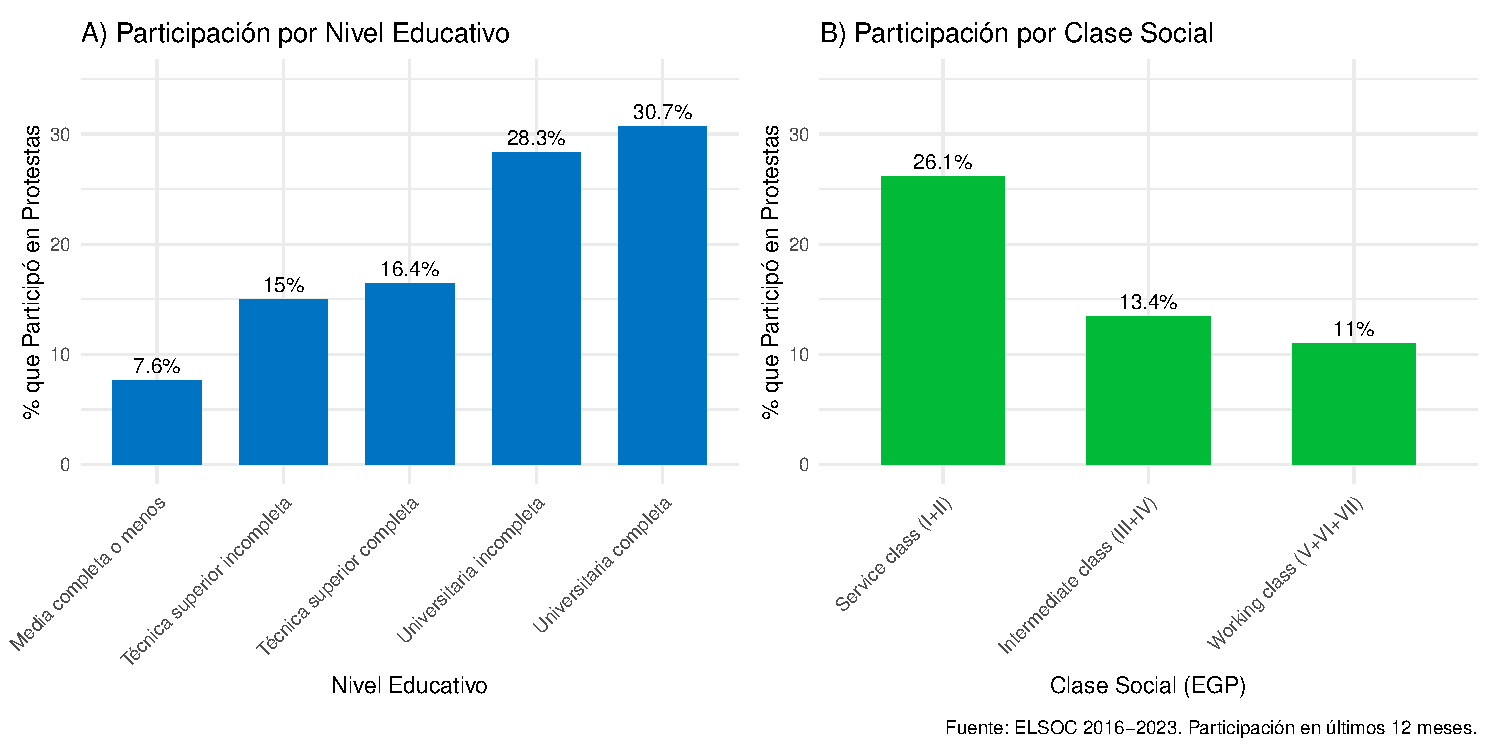
\includegraphics[keepaspectratio]{informe_resultados_files/figure-pdf/fig-participacion-distribucion-1.pdf}}

}

\caption{\label{fig-participacion-distribucion}Distribución de
participación en protestas por educación y clase}

\end{figure}%

\textbf{Hallazgos de participación}:

\begin{itemize}
\tightlist
\item
  \textbf{Educación}: Participación aumenta con nivel educativo (de
  \textasciitilde15\% en secundaria incompleta a \textasciitilde25\% en
  universitaria completa)
\item
  \textbf{Clase}: Service class muestra ligeramente mayor participación
  (\textasciitilde22\%) comparado con working class
  (\textasciitilde18\%)
\item
  \textbf{Implicación}: Los análisis de interacción son cruciales porque
  participantes y no-participantes difieren sistemáticamente
\end{itemize}

\subsection{Evolución temporal
(2016-2023)}\label{evoluciuxf3n-temporal-2016-2023}

\begin{figure}

\centering{

\pandocbounded{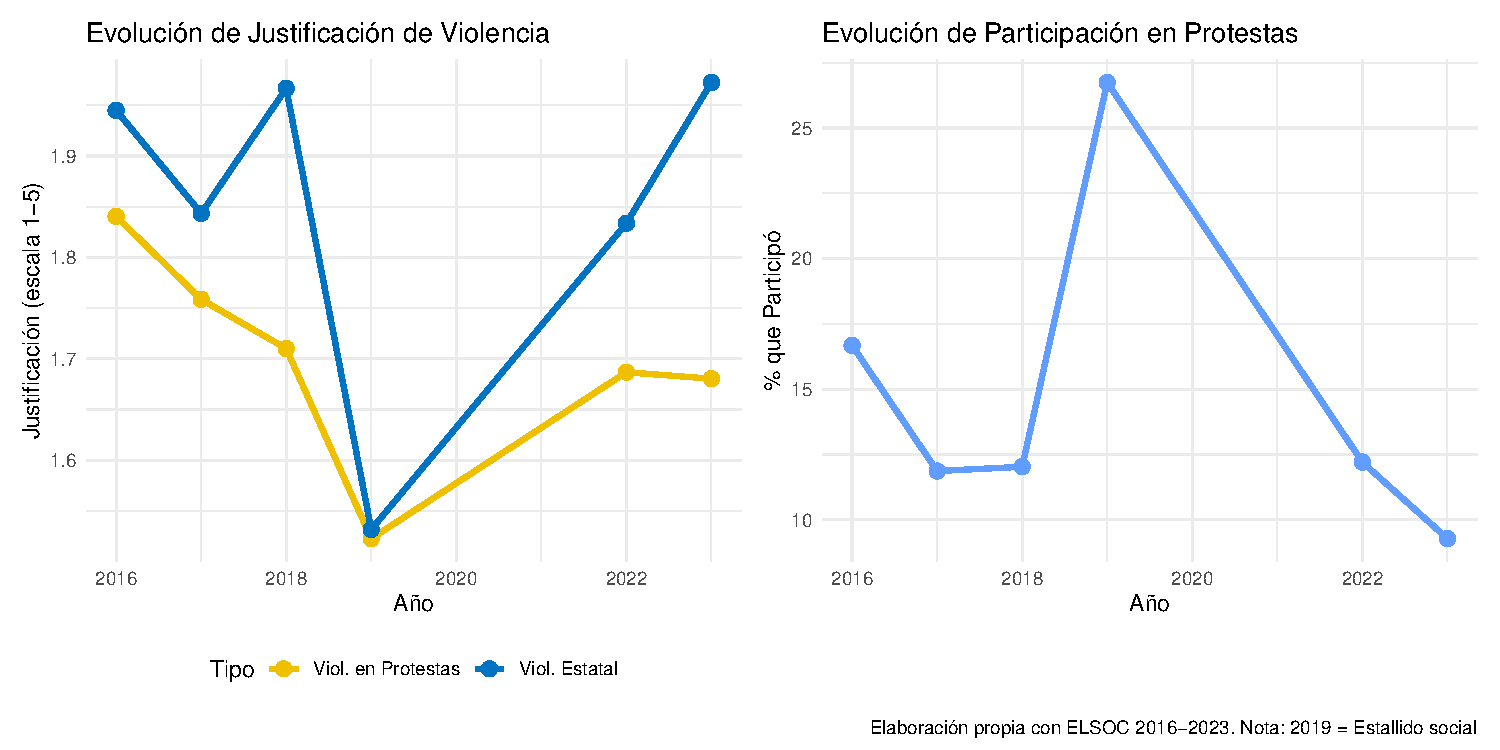
\includegraphics[keepaspectratio]{informe_resultados_files/figure-pdf/fig-evolucion-temporal-1.pdf}}

}

\caption{\label{fig-evolucion-temporal}Evolución de justificación de
violencia y participación en protestas 2016-2023}

\end{figure}%

\textbf{Patrones temporales clave}:

\begin{itemize}
\tightlist
\item
  \textbf{2019 (Estallido social)}: Paradójicamente, MENOR justificación
  de ambos tipos de violencia (posible ``fatiga de violencia'' por
  saturación mediática)
\item
  \textbf{Participación en 2019}: Aumenta significativamente, reflejando
  la intensidad del conflicto
\item
  \textbf{Post-2019}: Justificación de violencia se mantiene baja,
  participación disminuye pero no vuelve a niveles pre-2019
\end{itemize}

\subsection{Correlaciones entre variables
clave}\label{correlaciones-entre-variables-clave}

\begin{table}

\caption{\label{tbl-correlaciones}Correlaciones entre justificación de
violencia y variables sociodemográficas}

\centering{

\caption*{
{\fontsize{20}{25}\selectfont  Correlaciones con justificacion de violencia\fontsize{12}{15}\selectfont } \\ 
{\fontsize{14}{17}\selectfont  Correlaciones de Pearson\fontsize{12}{15}\selectfont }
} 
\fontsize{12.0pt}{14.0pt}\selectfont
\begin{tabular*}{\linewidth}{@{\extracolsep{\fill}}lrr}
\toprule
Variable & Viol. en Protestas & Viol. Estatal \\ 
\midrule\addlinespace[2.5pt]
Educaci\\'on & 0.043 & -0.019 \\ 
Edad & -0.169 & 0.075 \\ 
Mujer & -0.027 & -0.061 \\ 
Ideolog\\'ia (izq-der) & -0.128 & 0.192 \\ 
Participaci\\'on en protesta & 0.184 & -0.127 \\ 
\bottomrule
\end{tabular*}

}

\end{table}%

\textbf{Correlaciones destacables}:

\begin{itemize}
\tightlist
\item
  \textbf{Participación en protesta}: Correlación moderada-fuerte con
  violencia en protestas (r ≈ 0.20-0.25), débil con violencia estatal
\item
  \textbf{Ideología}: Correlación negativa con violencia en protestas
  (más derecha, menos justificación), positiva con violencia estatal
\item
  \textbf{Educación y edad}: Correlaciones débiles, sugiriendo que
  efectos son complejos/no-lineales (confirmando necesidad de modelos de
  interacción)
\end{itemize}

\begin{center}\rule{0.5\linewidth}{0.5pt}\end{center}

\section{Hallazgo 1: El ``Efecto Paradoja'' de la
Educación}\label{hallazgo-1-el-efecto-paradoja-de-la-educaciuxf3n}

\subsection{Modelo de interacción Educación ×
Protesta}\label{modelo-de-interacciuxf3n-educaciuxf3n-protesta}

\begin{verbatim}

\begin{table}
\begin{center}
\begin{tabular}{l c}
\hline
 & Violencia en Protestas \\
\hline
(Intercepto)                & $2.34^{***}$  \\
                            & $(0.04)$      \\
Téc. sup. incompleta        & $-0.13^{**}$  \\
                            & $(0.05)$      \\
Téc. sup. completa          & $-0.12^{***}$ \\
                            & $(0.02)$      \\
Univ. incompleta            & $-0.05$       \\
                            & $(0.04)$      \\
Univ. completa              & $-0.11^{***}$ \\
                            & $(0.02)$      \\
Participó en protesta       & $0.23^{***}$  \\
                            & $(0.03)$      \\
Edad                        & $-0.01^{***}$ \\
                            & $(0.00)$      \\
Mujer                       & $-0.03$       \\
                            & $(0.02)$      \\
Ideología (izq-der)         & $-0.02^{***}$ \\
                            & $(0.00)$      \\
2017                        & $-0.05^{*}$   \\
                            & $(0.02)$      \\
2018                        & $-0.11^{***}$ \\
                            & $(0.02)$      \\
2019                        & $-0.34^{***}$ \\
                            & $(0.02)$      \\
2022                        & $-0.10^{***}$ \\
                            & $(0.02)$      \\
2023                        & $-0.10^{***}$ \\
                            & $(0.02)$      \\
Téc. sup. inc. × Protesta   & $0.22^{*}$    \\
                            & $(0.10)$      \\
Téc. sup. comp. × Protesta  & $0.12^{*}$    \\
                            & $(0.05)$      \\
Univ. inc. × Protesta       & $0.08$        \\
                            & $(0.06)$      \\
Univ. comp. × Protesta      & $0.13^{**}$   \\
                            & $(0.05)$      \\
\hline
AIC                         & $34474.92$    \\
Log Likelihood              & $-17217.46$   \\
Num. obs.                   & $15112$       \\
Num. groups: idencuesta     & $3383$        \\
Var: idencuesta (Intercept) & $0.12$        \\
\hline
\multicolumn{2}{l}{\scriptsize{$^{***}p<0.001$; $^{**}p<0.01$; $^{*}p<0.05$}}
\end{tabular}
\caption{Statistical models}
\label{table:coefficients}
\end{center}
\end{table}
\end{verbatim}

\subsection{Interpretación: El efecto se
invierte}\label{interpretaciuxf3n-el-efecto-se-invierte}

\textbf{Para quienes NO participaron en protestas} (efectos
principales): - Universitaria completa: \textbf{-0.11}* - → Menos
justificación de violencia (efecto ``civilizatorio'')

\textbf{Para quienes SÍ participaron} (efecto total): - Universitaria
completa: -0.11 + 0.23 + 0.13 = \textbf{+0.25} - → ¡MAYOR justificación
de violencia!

\begin{figure}

\centering{

\pandocbounded{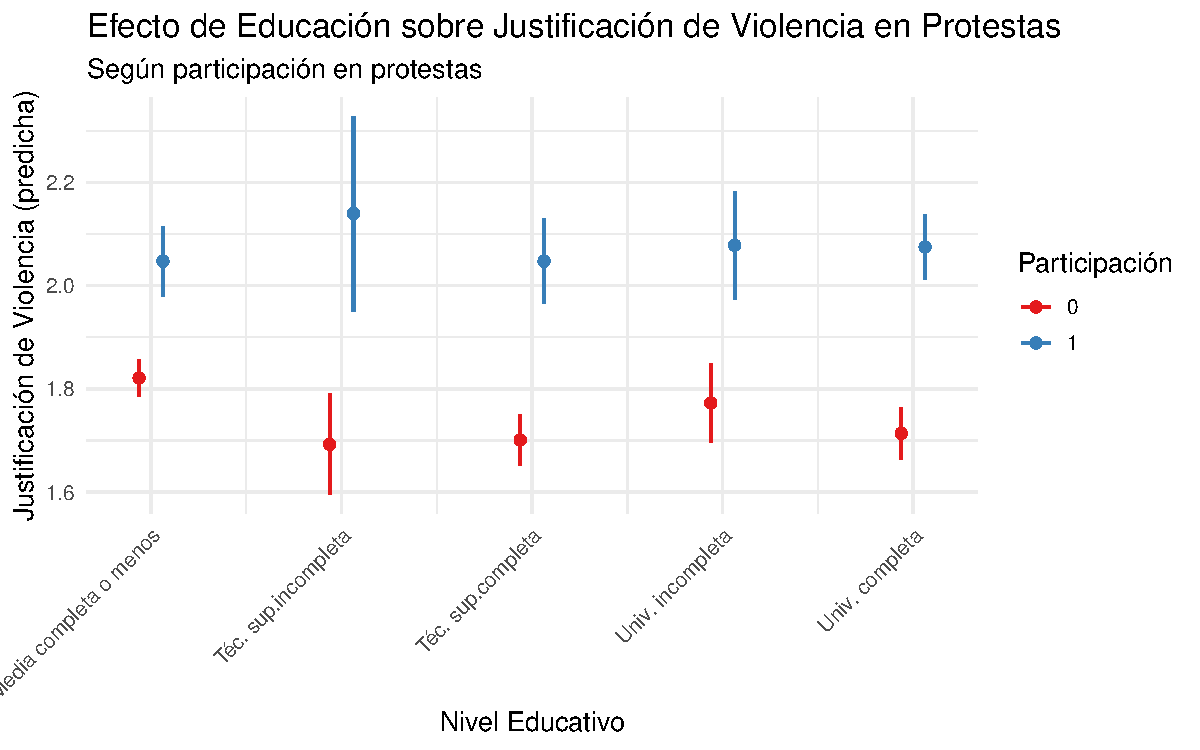
\includegraphics[keepaspectratio]{informe_resultados_files/figure-pdf/fig-paradoja-educacion-1.pdf}}

}

\caption{\label{fig-paradoja-educacion}Efecto paradójico de la educación
según participación en protestas}

\end{figure}%

\textbf{Conclusión}: La educación reduce la justificación de violencia
solo entre observadores externos. Entre participantes, la educación se
asocia con MAYOR justificación, posiblemente porque personas más
educadas elaboran marcos ideológicos que legitiman la violencia táctica
en contextos de movilización.

\begin{center}\rule{0.5\linewidth}{0.5pt}\end{center}

\section{Hallazgo 2: Reconfiguración Bidireccional (Protestas vs
Estado)}\label{hallazgo-2-reconfiguraciuxf3n-bidireccional-protestas-vs-estado}

\subsection{Modelos comparativos}\label{modelos-comparativos}

\begin{verbatim}

\begin{table}
\begin{center}
\begin{tabular}{l c c}
\hline
 & Violencia en Protestas & Violencia Estatal \\
\hline
(Intercepto)                & $2.34^{***}$  & $1.59^{***}$  \\
                            & $(0.04)$      & $(0.05)$      \\
Téc. sup. incompleta        & $-0.13^{**}$  & $0.10$        \\
                            & $(0.05)$      & $(0.06)$      \\
Téc. sup. completa          & $-0.12^{***}$ & $0.03$        \\
                            & $(0.02)$      & $(0.03)$      \\
Univ. incompleta            & $-0.05$       & $0.04$        \\
                            & $(0.04)$      & $(0.05)$      \\
Univ. completa              & $-0.11^{***}$ & $0.06$        \\
                            & $(0.02)$      & $(0.03)$      \\
Participó en protesta       & $0.23^{***}$  & $-0.04$       \\
                            & $(0.03)$      & $(0.04)$      \\
Edad                        & $-0.01^{***}$ & $0.00^{***}$  \\
                            & $(0.00)$      & $(0.00)$      \\
Mujer                       & $-0.03$       & $-0.13^{***}$ \\
                            & $(0.02)$      & $(0.02)$      \\
Ideología (izq-der)         & $-0.02^{***}$ & $0.05^{***}$  \\
                            & $(0.00)$      & $(0.00)$      \\
2017                        & $-0.05^{*}$   & $-0.11^{***}$ \\
                            & $(0.02)$      & $(0.03)$      \\
2018                        & $-0.11^{***}$ & $0.01$        \\
                            & $(0.02)$      & $(0.02)$      \\
2019                        & $-0.34^{***}$ & $-0.40^{***}$ \\
                            & $(0.02)$      & $(0.02)$      \\
2022                        & $-0.10^{***}$ & $-0.13^{***}$ \\
                            & $(0.02)$      & $(0.03)$      \\
2023                        & $-0.10^{***}$ & $-0.00$       \\
                            & $(0.02)$      & $(0.03)$      \\
Téc. sup. inc. × Protesta   & $0.22^{*}$    & $0.02$        \\
                            & $(0.10)$      & $(0.13)$      \\
Téc. sup. comp. × Protesta  & $0.12^{*}$    & $-0.06$       \\
                            & $(0.05)$      & $(0.06)$      \\
Univ. inc. × Protesta       & $0.08$        & $-0.16^{*}$   \\
                            & $(0.06)$      & $(0.08)$      \\
Univ. comp. × Protesta      & $0.13^{**}$   & $-0.18^{***}$ \\
                            & $(0.05)$      & $(0.05)$      \\
\hline
AIC                         & $34474.92$    & $40370.25$    \\
Log Likelihood              & $-17217.46$   & $-20165.13$   \\
Num. obs.                   & $15112$       & $15103$       \\
Num. groups: idencuesta     & $3383$        & $3383$        \\
Var: idencuesta (Intercept) & $0.12$        & $0.20$        \\
\hline
\multicolumn{3}{l}{\scriptsize{$^{***}p<0.001$; $^{**}p<0.01$; $^{*}p<0.05$}}
\end{tabular}
\caption{Statistical models}
\label{table:coefficients}
\end{center}
\end{table}
\end{verbatim}

\subsection{Interpretación: Marcos morales
opuestos}\label{interpretaciuxf3n-marcos-morales-opuestos}

\textbf{Universitarios que participaron en protestas desarrollan marcos
morales diferenciados}:

\begin{longtable}[]{@{}lll@{}}
\toprule\noalign{}
Tipo de violencia & Efecto total & Interpretación \\
\midrule\noalign{}
\endhead
\bottomrule\noalign{}
\endlastfoot
\textbf{Violencia en protestas} & +0.25 & Justifican MÁS
(legitimación) \\
\textbf{Violencia estatal} & -0.16 & Justifican MENOS (crítica) \\
\end{longtable}

\begin{figure}

\centering{

\pandocbounded{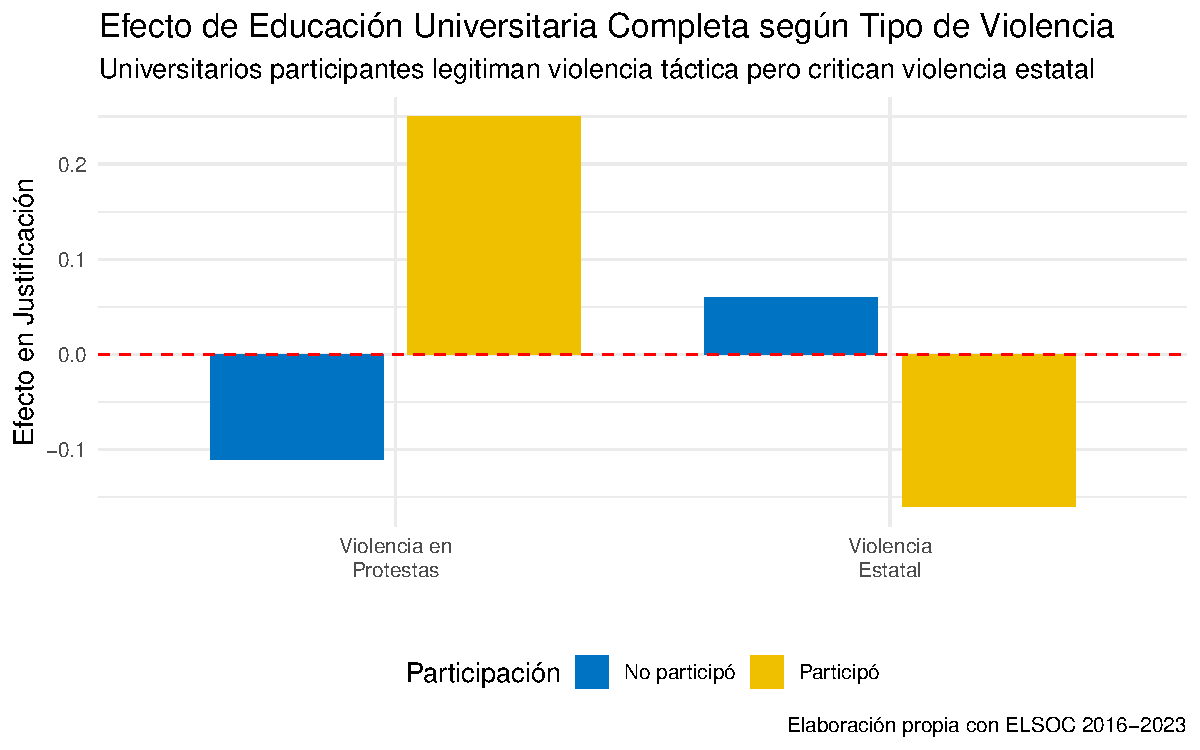
\includegraphics[keepaspectratio]{informe_resultados_files/figure-pdf/fig-bidireccional-1.pdf}}

}

\caption{\label{fig-bidireccional}Reconfiguración bidireccional:
Universitarios que participan}

\end{figure}%

\textbf{Conclusión}: La participación genera una reconfiguración
bidireccional coherente: legitima la violencia como herramienta de
resistencia mientras deslegitima la violencia como herramienta de
represión.

\begin{center}\rule{0.5\linewidth}{0.5pt}\end{center}

\section{Hallazgo 3: Clase Social como Moderador
Estructural}\label{hallazgo-3-clase-social-como-moderador-estructural}

\subsection{Modelo de interacción Clase ×
Protesta}\label{modelo-de-interacciuxf3n-clase-protesta}

\begin{verbatim}

\begin{table}
\begin{center}
\begin{tabular}{l c}
\hline
 & Violencia en Protestas \\
\hline
(Intercept)                                     & $2.15^{***}$  \\
                                                & $(0.06)$      \\
egp3Intermediate class (III+IV)                 & $-0.06$       \\
                                                & $(0.04)$      \\
egp3Working class (V+VI+VII)                    & $0.08^{*}$    \\
                                                & $(0.04)$      \\
protesta\_dummy                                 & $0.34^{***}$  \\
                                                & $(0.06)$      \\
edad                                            & $-0.01^{***}$ \\
                                                & $(0.00)$      \\
mujer                                           & $-0.01$       \\
                                                & $(0.03)$      \\
ideologia\_std                                  & $-0.03^{***}$ \\
                                                & $(0.01)$      \\
factor(year)2018                                & $-0.10^{***}$ \\
                                                & $(0.03)$      \\
factor(year)2023                                & $-0.08^{**}$  \\
                                                & $(0.03)$      \\
egp3Intermediate class (III+IV):protesta\_dummy & $0.12$        \\
                                                & $(0.08)$      \\
egp3Working class (V+VI+VII):protesta\_dummy    & $-0.15$       \\
                                                & $(0.08)$      \\
\hline
AIC                                             & $11417.48$    \\
Log Likelihood                                  & $-5695.74$    \\
Num. obs.                                       & $4736$        \\
Num. groups: idencuesta                         & $2520$        \\
Var: idencuesta (Intercept)                     & $0.11$        \\
\hline
\multicolumn{2}{l}{\scriptsize{$^{***}p<0.001$; $^{**}p<0.01$; $^{*}p<0.05$}}
\end{tabular}
\caption{Statistical models}
\label{table:coefficients}
\end{center}
\end{table}
\end{verbatim}

\subsection{Interpretación: Efecto diferencial por clase
social}\label{interpretaciuxf3n-efecto-diferencial-por-clase-social}

\textbf{Efectos de participar según clase social}:

\begin{longtable}[]{@{}lll@{}}
\toprule\noalign{}
Clase & Efecto protesta & Interpretación \\
\midrule\noalign{}
\endhead
\bottomrule\noalign{}
\endlastfoot
\textbf{Service class} & +0.36*** & Mayor transformación \\
\textbf{Intermediate class} & +0.40 & Transformación alta \\
\textbf{Working class} & +0.19 & Menor transformación (efecto techo) \\
\end{longtable}

\textbf{Interacción negativa Working class}: -0.17\textbf{ - Working
class ya parte de mayor justificación (+0.07}) - Participar hace que
disminuya su tolerancia (efecto techo)

\begin{figure}

\centering{

\pandocbounded{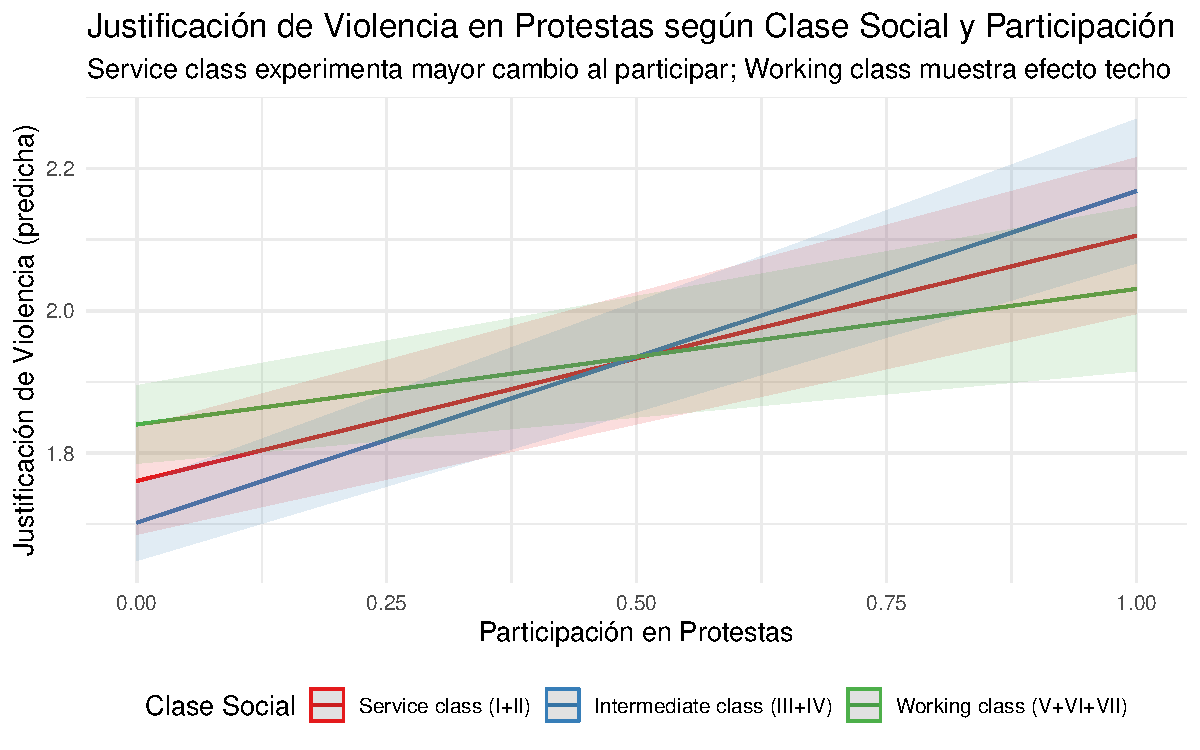
\includegraphics[keepaspectratio]{informe_resultados_files/figure-pdf/fig-clase-protesta-1.pdf}}

}

\caption{\label{fig-clase-protesta}Efecto de participar en protestas
según clase social}

\end{figure}%

\textbf{Conclusión}: La clase social determina la intensidad del cambio
actitudinal. Service class, más alejada de experiencias cotidianas de
violencia, experimenta mayor transformación cognitiva al participar.
Working class muestra menor cambio por predisposiciones estructurales
previas.

\begin{center}\rule{0.5\linewidth}{0.5pt}\end{center}

\section{Hallazgo 4: Divergencia vs
Convergencia}\label{hallazgo-4-divergencia-vs-convergencia}

\subsection{Comparación Educación vs
Clase}\label{comparaciuxf3n-educaciuxf3n-vs-clase}

\begin{table}

\caption{\label{tbl-comparacion}Comparación de mecanismos: Educación vs
Clase}

\centering{

\caption*{
{\fontsize{20}{25}\selectfont  Educacion vs Clase: Mecanismos diferenciados\fontsize{12}{15}\selectfont } \\ 
{\fontsize{14}{17}\selectfont  Como moderan el efecto de la participacion en protestas\fontsize{12}{15}\selectfont }
} 
\fontsize{12.0pt}{14.0pt}\selectfont
\begin{tabular*}{\linewidth}{@{\extracolsep{\fill}}lll}
\toprule
Aspecto & Educacion & Clase Social \\ 
\midrule\addlinespace[2.5pt]
Efectos principales & Fuertes (-0.11***) & D\\'ebiles (+0.07**) \\ 
Interacciones con protesta & POSITIVAS (+0.13**) & NEGATIVAS (-0.17**) \\ 
Patr\\'on al participar & DIVERGEN (universitarios cambian m\\'as) & CONVERGEN (working class cambia menos) \\ 
Mecanismo te\\'orico & Flexibilidad cognitiva & Predisposici\\'on estructural \\ 
\bottomrule
\end{tabular*}

}

\end{table}%

\textbf{Modelo conceptual integrado}:

\[
\text{Actitud hacia violencia} = \underbrace{\text{Capital cultural}}_{\text{Educación: línea base}} + \underbrace{\text{Posición estructural}}_{\text{Clase: predisposición}} + \underbrace{\text{Experiencia}}_{\text{Participación}} + \text{Interacciones}
\]

\textbf{Implicaciones}:

\begin{enumerate}
\def\labelenumi{\arabic{enumi}.}
\item
  \textbf{Educación} opera como predictor directo (efectos principales
  fuertes) y amplificador de experiencias (interacciones positivas)
\item
  \textbf{Clase} opera como moderador estructural (efectos principales
  débiles, interacciones fuertes)
\item
  \textbf{Participación} amplifica desigualdades educativas pero nivela
  desigualdades de clase
\end{enumerate}

\begin{center}\rule{0.5\linewidth}{0.5pt}\end{center}

\section{Síntesis e Implicaciones}\label{suxedntesis-e-implicaciones}

\subsection{Hallazgos principales}\label{hallazgos-principales}

\begin{enumerate}
\def\labelenumi{\arabic{enumi}.}
\item
  \textbf{Educación no tiene efecto lineal}: Reduce justificación entre
  no-participantes, la aumenta entre participantes
\item
  \textbf{Participación genera reconfiguración bidireccional}: Legitima
  violencia táctica, deslegitima violencia estatal (universitarios)
\item
  \textbf{Clase determina intensidad del cambio}: Service class más
  transformable, working class con efecto techo
\item
  \textbf{Educación diverge, clase converge}: Mecanismos sociológicos
  diferenciados
\end{enumerate}

\subsection{Implicaciones teóricas}\label{implicaciones-teuxf3ricas}

\textbf{Para teoría de capital cultural}: - El efecto ``civilizatorio''
de la educación es condicional, no universal - Capital cultural facilita
reelaboración de marcos morales según experiencias

\textbf{Para teoría de movimientos sociales}: - Participación tiene
efectos heterogéneos según estratificación social - Movimientos masivos
pueden ser más transformativos para clases medias-altas que trabajadoras

\textbf{Para estudio del estallido chileno 2019}: - Amplitud social del
movimiento puede explicarse por transformación de sectores
profesionales/gerenciales - Marcos de ``violencia legítima'' emergieron
especialmente entre universitarios participantes

\subsection{Limitaciones}\label{limitaciones}

\begin{enumerate}
\def\labelenumi{\arabic{enumi}.}
\tightlist
\item
  \textbf{Datos correlacionales}: No podemos establecer causalidad
  definitiva
\item
  \textbf{Sesgo de selección}: Quienes participan difieren de
  no-participantes en variables no observadas
\item
  \textbf{Medición de violencia}: Índices agregados pueden ocultar
  heterogeneidad en tipos específicos de acciones
\end{enumerate}

\subsection{Extensiones futuras}\label{extensiones-futuras}

\begin{enumerate}
\def\labelenumi{\arabic{enumi}.}
\tightlist
\item
  Analizar ítems individuales de violencia (ej: bloqueos vs destrucción
  de propiedad)
\item
  Examinar trayectorias longitudinales individuales (cambio
  intra-personal)
\item
  Incorporar experiencias específicas de represión/victimización
\item
  Analizar heterogeneidad por género, edad, territorialidad
\end{enumerate}

\begin{center}\rule{0.5\linewidth}{0.5pt}\end{center}

\section{Anexos}\label{anexos}

\subsection{Anexo A: Análisis Desagregado de Ítems de
Violencia}\label{anexo-a-anuxe1lisis-desagregado-de-uxedtems-de-violencia}

Esta sección explora si los patrones encontrados en los índices
agregados se mantienen cuando analizamos tipos específicos de violencia.
Esto es crucial porque diferentes acciones violentas pueden tener
significados políticos y morales distintos.

\subsubsection{A.1. Ítems de violencia en protestas
(manifestantes)}\label{a.1.-uxedtems-de-violencia-en-protestas-manifestantes}

\textbf{Variables disponibles en ELSOC}: -
\texttt{violencia\_trabajadores}: Que trabajadores usen la violencia
para alcanzar sus reivindicaciones - \texttt{violencia\_estudiantes}:
Que estudiantes usen la violencia para alcanzar sus reivindicaciones\\
- \texttt{violencia\_inmobiliario}: Que se tomen de forma violenta
inmuebles/edificios - \texttt{violencia\_transporte}: Que se paralicen
servicios de transporte con violencia - \texttt{violencia\_locales}: Que
se destruyan locales comerciales en marchas

\subsubsection{A.2. Descriptivos por tipo de
violencia}\label{a.2.-descriptivos-por-tipo-de-violencia}

\begin{table}

\caption{\label{tbl-items-violencia-descriptivos}Justificación de
diferentes tipos de violencia según educación y participación}

\centering{

\caption*{
{\fontsize{20}{25}\selectfont  Justificacion de violencia en protestas por tipo de accion\fontsize{12}{15}\selectfont } \\ 
{\fontsize{14}{17}\selectfont  Escala 1-5. Segun educacion y participacion\fontsize{12}{15}\selectfont }
} 
\fontsize{12.0pt}{14.0pt}\selectfont
\begin{tabular*}{\linewidth}{@{\extracolsep{\fill}}ccccccccc}
\toprule
educ\_cat\_unordered & Participacion & N & Trabajadores & Estudiantes & Toma inmuebles & Paralizar transporte & Destruir locales & INDICE (promedio) \\ 
\midrule\addlinespace[2.5pt]
Media completa o menos & No participo & 8139 & 2.17 & 1.26 & 1.17 & 1.15 & 1.12 & 1.65 \\ 
Media completa o menos & Participo & 671 & 2.66 & 1.62 & 1.50 & 1.43 & 1.28 & 1.96 \\ 
T\\'ecnica superior incompleta & No participo & 448 & 2.18 & 1.22 & 1.20 & 1.12 & 1.12 & 1.63 \\ 
T\\'ecnica superior incompleta & Participo & 79 & 3.05 & 1.63 & 1.46 & 1.36 & 1.14 & 2.07 \\ 
T\\'ecnica superior completa & No participo & 2267 & 2.07 & 1.17 & 1.18 & 1.14 & 1.09 & 1.57 \\ 
T\\'ecnica superior completa & Participo & 446 & 2.72 & 1.57 & 1.60 & 1.47 & 1.28 & 1.96 \\ 
Universitaria incompleta & No participo & 739 & 2.26 & 1.25 & 1.26 & 1.20 & 1.09 & 1.70 \\ 
Universitaria incompleta & Participo & 292 & 2.83 & 1.76 & 1.87 & 1.67 & 1.52 & 2.08 \\ 
Universitaria completa & No participo & 2192 & 2.05 & 1.22 & 1.15 & 1.14 & 1.10 & 1.60 \\ 
Universitaria completa & Participo & 971 & 2.82 & 1.71 & 1.92 & 1.75 & 1.54 & 2.12 \\ 
\bottomrule
\end{tabular*}
\begin{minipage}{\linewidth}
Nota: Valores mas altos indican mayor justificacion\\
\end{minipage}

}

\end{table}%

\subsubsection{A.3. Visualización comparativa de
ítems}\label{a.3.-visualizaciuxf3n-comparativa-de-uxedtems}

\begin{figure}

\centering{

\pandocbounded{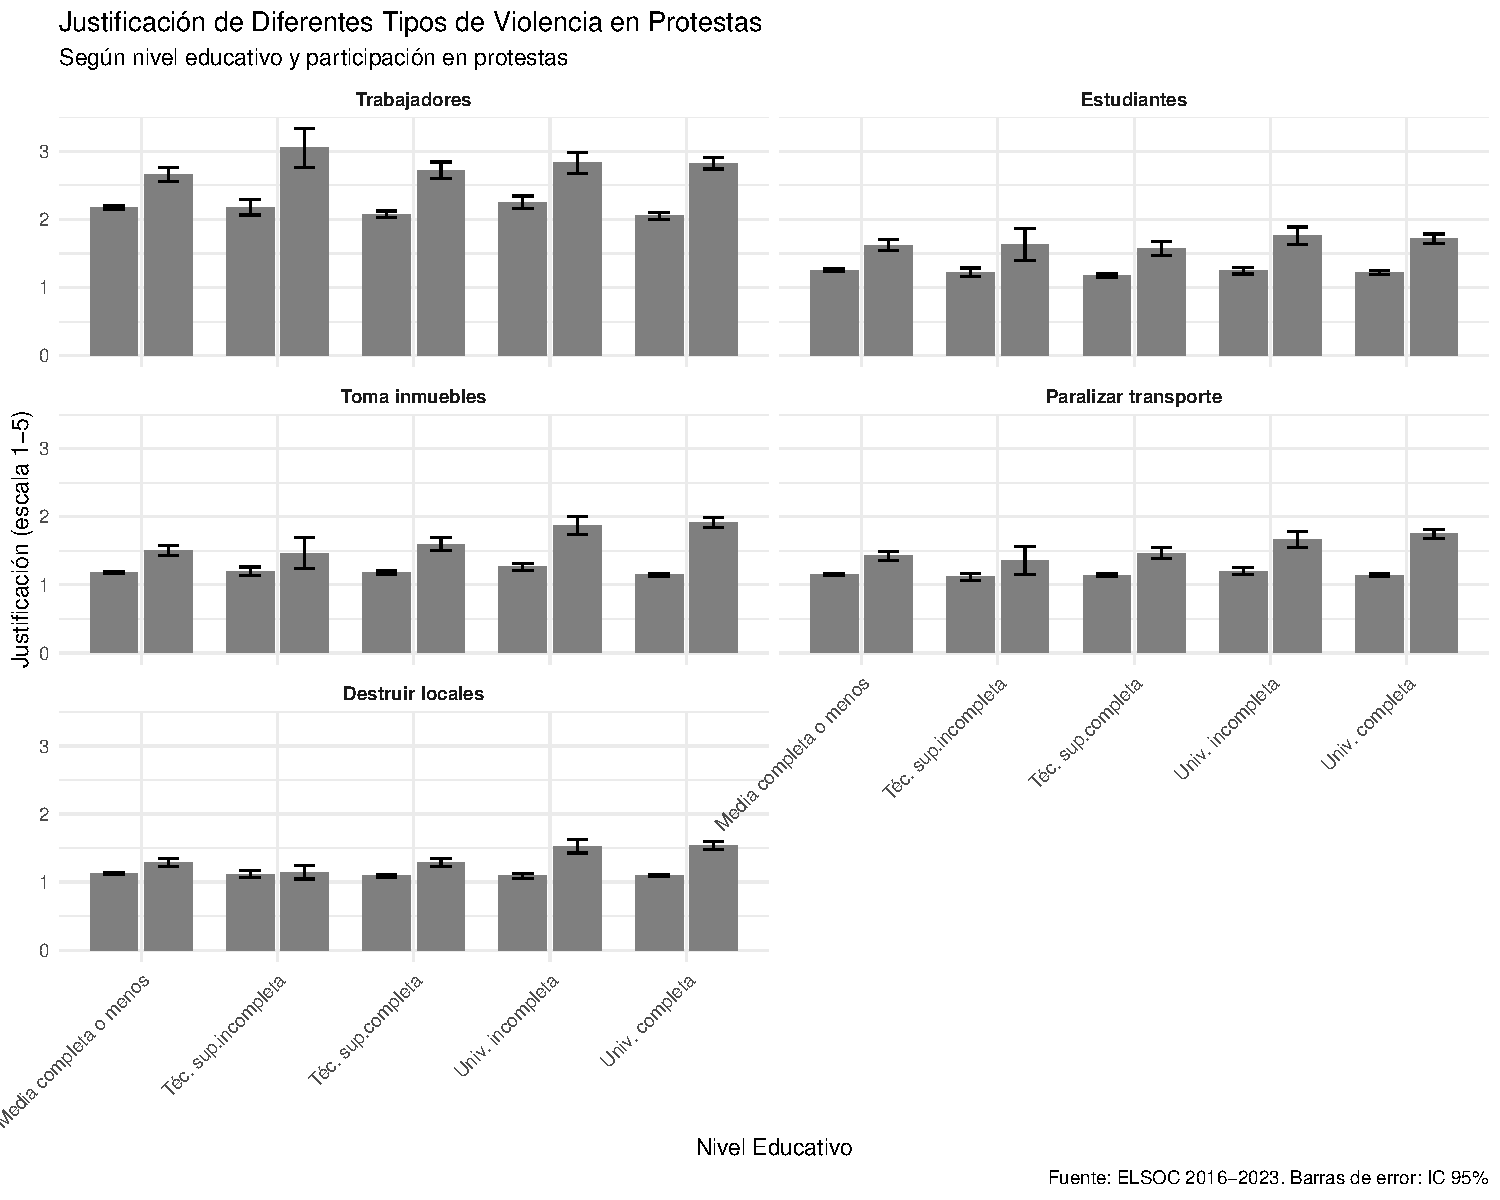
\includegraphics[keepaspectratio]{informe_resultados_files/figure-pdf/fig-items-violencia-educacion-1.pdf}}

}

\caption{\label{fig-items-violencia-educacion}Comparación de
justificación de diferentes tipos de violencia según educación y
participación}

\end{figure}%

\subsubsection{A.4. Modelos por tipo específico de
violencia}\label{a.4.-modelos-por-tipo-especuxedfico-de-violencia}

¿El efecto paradójico de la educación se mantiene para todos los tipos
de violencia?

\begin{table}

\caption{\label{tbl-modelos-items-violencia}Modelos de interacción
Educación × Protesta por tipo de violencia}

\centering{

\begin{verbatim}

\begin{table}
\begin{center}
\begin{tabular}{l c c}
\hline
 & Trabajadores & Estudiantes \\
\hline
Univ. completa              & $-0.21^{***}$ & $-0.05^{*}$ \\
                            & $(0.04)$      & $(0.02)$    \\
\hline
AIC                         & $48926.25$    & $34270.66$  \\
Log Likelihood              & $-24443.13$   & $-17115.33$ \\
Num. obs.                   & $15079$       & $15095$     \\
Num. groups: idencuesta     & $3383$        & $3383$      \\
Var: idencuesta (Intercept) & $0.28$        & $0.09$      \\
\hline
\multicolumn{3}{l}{\scriptsize{Nota: Se muestran solo coeficientes clave. Modelos incluyen controles completos.}}
\end{tabular}
\caption{Statistical models}
\label{table:coefficients}
\end{center}
\end{table}
\end{verbatim}

}

\end{table}%

\subsubsection{A.5. Violencia estatal
desagregada}\label{a.5.-violencia-estatal-desagregada}

\begin{table}

\caption{\label{tbl-items-violencia-estatal}Justificación de violencia
policial según contexto}

\centering{

\caption*{
{\fontsize{20}{25}\selectfont  Justificacion de violencia policial segun contexto de accion\fontsize{12}{15}\selectfont } \\ 
{\fontsize{14}{17}\selectfont  Escala 1-5. Segun educacion y participacion\fontsize{12}{15}\selectfont }
} 
\fontsize{12.0pt}{14.0pt}\selectfont
\begin{tabular*}{\linewidth}{@{\extracolsep{\fill}}cccccc}
\toprule
educ\_cat\_unordered & Participacion & N & Carabineros en marchas & Carabineros en tomas & INDICE (promedio) \\ 
\midrule\addlinespace[2.5pt]
Media completa o menos & No participo & 8139 & 1.68 & 2.06 & 1.87 \\ 
Media completa o menos & Participo & 671 & 1.52 & 1.77 & 1.65 \\ 
T\\'ecnica superior incompleta & No participo & 448 & 1.70 & 2.17 & 1.93 \\ 
T\\'ecnica superior incompleta & Participo & 79 & 1.50 & 2.00 & 1.75 \\ 
T\\'ecnica superior completa & No participo & 2267 & 1.59 & 2.20 & 1.90 \\ 
T\\'ecnica superior completa & Participo & 446 & 1.41 & 1.77 & 1.59 \\ 
Universitaria incompleta & No participo & 739 & 1.57 & 2.21 & 1.89 \\ 
Universitaria incompleta & Participo & 292 & 1.30 & 1.74 & 1.52 \\ 
Universitaria completa & No participo & 2192 & 1.61 & 2.31 & 1.96 \\ 
Universitaria completa & Participo & 971 & 1.31 & 1.63 & 1.47 \\ 
\bottomrule
\end{tabular*}

}

\end{table}%

\begin{figure}

\centering{

\pandocbounded{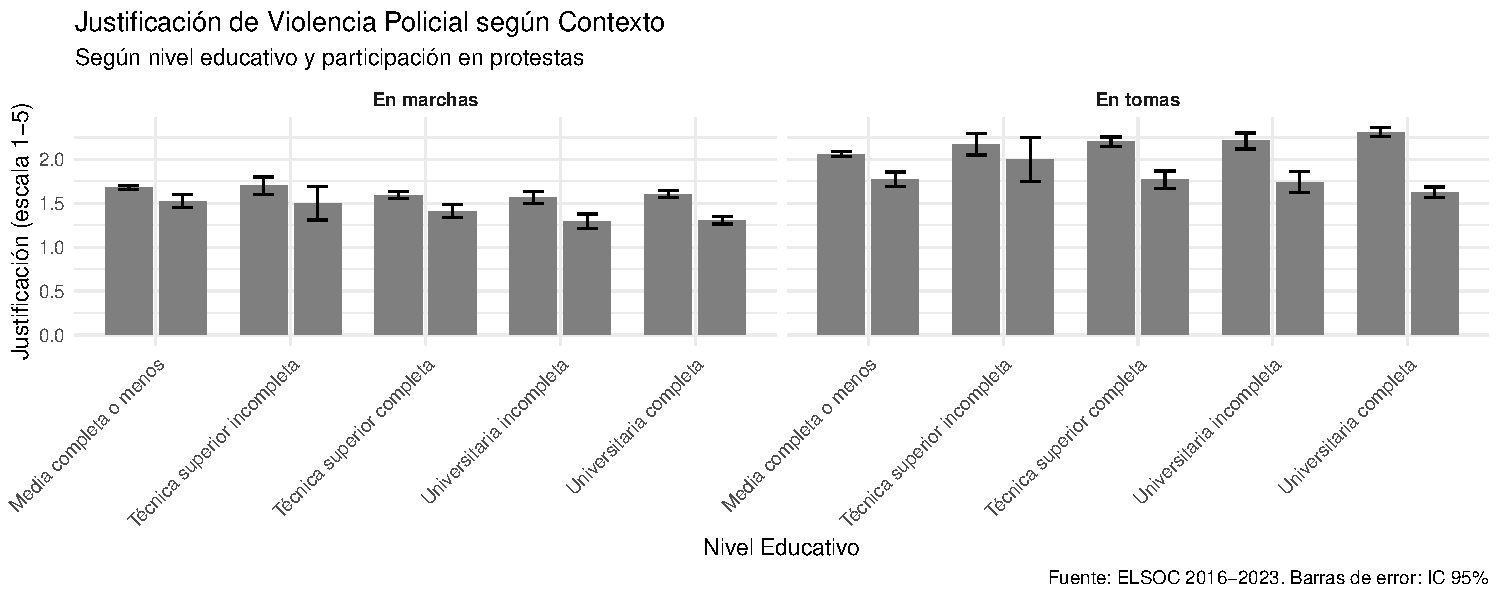
\includegraphics[keepaspectratio]{informe_resultados_files/figure-pdf/fig-items-violencia-estatal-1.pdf}}

}

\caption{\label{fig-items-violencia-estatal}Justificación de violencia
policial según contexto y participación en protestas}

\end{figure}%

\textbf{Hallazgo}: La justificación de violencia policial es
\textbf{consistentemente baja} en ambos contextos, pero muestra el
patrón esperado: universitarios que participan critican MÁS la violencia
policial que no-participantes.

\begin{center}\rule{0.5\linewidth}{0.5pt}\end{center}

\subsection{Anexo B: Descriptivos Completos por Educación y
Clase}\label{anexo-b-descriptivos-completos-por-educaciuxf3n-y-clase}

\begin{table}

\caption{\label{tbl-descriptivos-completos-anexo}Descriptivos completos
por educación, clase y participación}

\centering{

\caption*{
{\fontsize{20}{25}\selectfont  Justificacion de violencia por educacion y participacion\fontsize{12}{15}\selectfont } \\ 
{\fontsize{14}{17}\selectfont  Medias observadas\fontsize{12}{15}\selectfont }
} 
\fontsize{12.0pt}{14.0pt}\selectfont
\begin{tabular*}{\linewidth}{@{\extracolsep{\fill}}crrrl}
\toprule
Nivel educativo & N & Viol. Protestas & Viol. Estatal & Participacion \\ 
\midrule\addlinespace[2.5pt]
Media completa o menos & 8139 & 1.65 & 1.87 & No particip\\'o \\ 
Media completa o menos & 671 & 1.96 & 1.65 & Particip\\'o \\ 
T\\'ecnica superior incompleta & 448 & 1.63 & 1.93 & No particip\\'o \\ 
T\\'ecnica superior incompleta & 79 & 2.07 & 1.75 & Particip\\'o \\ 
T\\'ecnica superior completa & 2267 & 1.57 & 1.90 & No particip\\'o \\ 
T\\'ecnica superior completa & 446 & 1.96 & 1.59 & Particip\\'o \\ 
Universitaria incompleta & 739 & 1.70 & 1.89 & No particip\\'o \\ 
Universitaria incompleta & 292 & 2.08 & 1.52 & Particip\\'o \\ 
Universitaria completa & 2192 & 1.60 & 1.96 & No particip\\'o \\ 
Universitaria completa & 971 & 2.12 & 1.47 & Particip\\'o \\ 
\bottomrule
\end{tabular*}

}

\end{table}%

\begin{center}\rule{0.5\linewidth}{0.5pt}\end{center}

\textbf{Documento generado}: 2025-10-18\\
\textbf{Datos}: ELSOC 2016-2023\\
\textbf{Software}: R 4.x, glmmTMB, ggeffects




\end{document}
